\section{Risk Mitigation}

Nel processo di “\textit{Risk Mitigation}” vengono analizzate le contromisure
raccomandate dal team di
assessment e poi selezionate e implementate quelle che presentano il
miglior rapporto costi/benefici.
Solitamente si adotta la modalità degli “\textbf{Attack Tree}”
(approcci qualitativi).
Più nel dettaglio distinguiamo:

\begin{itemize}
    \item Approcci \textbf{qualitativi}: Analisi degli scenari che possono
          realizzarsi all'interno di un sistema.
          Lo scopo è quello di individuare le possibili minacce e il livello di
          rischio associato ad ogni
          risorsa che compone il sistema. Vengono chiamati “Attack Tree” perché
          l'analisi dei
          possibili attacchi viene effettuata per mezzo della costruzione di alberi.
    \item Approcci \textbf{quantitativi} (Indici economici): Quantificazione di
          tutte le grandezze necessarie
          per una valutazione dei rischi con l'obiettivo di determinare,
          attraverso l'uso di una serie
          d'indici, la convenienza economica di un investimento in sicurezza.
\end{itemize}

\subsection{Attack Tree}

Gli \textit{Attack Trees} sono diagrammi concettuali che mostrano come una risorsa
o un obiettivo, potrebbe essere
attaccata.
Gli Attack Trees sono diagrammi multilivello costituiti da una radice, foglie e
figli. Dal basso verso l'alto, i nodi
figli sono condizioni che devono essere soddisfatte per rendere vero il nodo
genitore diretto; quando la radice è
soddisfatta, l'attacco è completo. Ogni nodo può essere soddisfatto solo dai
suoi nodi figli diretti . Un nodo può
essere figlio di un altro nodo; in tal caso, diventa logico che sia necessario
eseguire più passaggi per attuare un
attacco. Un attacco descritto in un nodo può richiedere che uno o più dei molti
attacchi descritti nei nodi figli siano
soddisfatti. si possono creare e verificare condizioni di OR o di AND lungo
l'albero.

Abbiamo quindi:

\begin{itemize}
    \item Radice: rappresenta l'asset che è oggetto dell'attacco,
    \item Nodi: sono possibili percorsi dell'attaccante per effettuare l'attacco.
          I nodi non foglie possono essere nodi AND, si devono eseguire entrambi
          gli attacchi per raggiungere il nodo, o nodi OR, dove ogni singolo
          percorso è un attacco.
\end{itemize}

\begin{figure}[H]
    \centering
    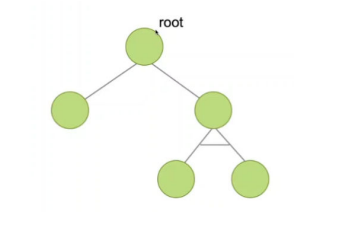
\includegraphics[width=8cm, keepaspectratio]{capitoli/risks/imgs/atree.png}
    \caption{Questa immagine rappresenta un Attack Tree.}
\end{figure}

Gli alberi di difesa (\textbf{Defense Tree}) sono un'estensione degli
Attack Trees (nodi quadrati). Si costruiscono per capire
quali sono le possibili contromisure da adottare.
Considerando tutte queste possibilità di un eventuale attacco,
devo definire le contromisure adatte per la protezione
dell'asset, tenendo sempre presente l'attack tree.
Un metodo piuttosto semplice prevede di mettere gli attacchi
in ordine di importanza e scegliere le contromisure da
adottare in base ad una certa priorità: per esempio in base
alla pericolosità, al costo, ecc.

\begin{figure}[H]
    \centering
    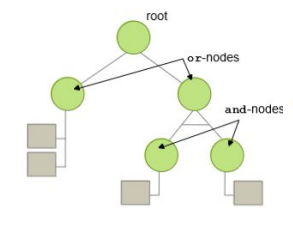
\includegraphics[width=8cm, keepaspectratio]{capitoli/risks/imgs/dtree.png}
    \caption{Questa immagine rappresenta un Defense Tree.}
\end{figure}

\subsection{Indici Economici}

\paragraph{SLE.}
La \textit{Single Loss Exposure} (\textbf{SLE}) rappresenta una misura della
perdita di un'impresa da un singolo
evento di minaccia e può essere calcolata utilizzando la seguente formula:

\[
    SLE = AV \times  EF
\]

Dove l'\textit{Asset Value} (\textit{AV}) è il costo di creazione, sviluppo,
supporto, sostituzione e proprietà di un bene;
l'\textit{Exposure Factor} (\textbf{EF}) rappresenta una misura dell'entità della
perdita o dell'impatto sul
valore di un'attività derivante da un evento di minaccia.

\paragraph{ALE.}
The \textit{Annualized Loss Expectancy} (\textbf{ALE}) è la perdita finanziaria
annuale prevista di un'impresa che
può essere attribuita a una minaccia.
Può essere calcolata utilizzando la seguente formula:

\[
    ALE = SLE \times ARO
\]

Dove \textit{Annualized Rate of Occurrence} (\textbf{ARO}) è un numero
che rappresenta il numero stimato di eventi annuali di una
minaccia. Questo è il costo da proteggere.

\paragraph{ROI.}
L'indicatore \textit{Return on Investment} (\textbf{ROI}) è dato da:

\[
    ROI = \frac{(ALE \times RM) - CSI}{CSI}
\]

Dove \(RM\) è il rischio mitigato (Risk Mitigated) da una
contromisura, rappresenta l'efficacia di una contromisura nel
mitigare il rischio di perdita derivante dallo sfruttamento di una
vulnerabilità; \(CSI\) è il costo dell'investimento in sicurezza
(Cost of Security Investment) che un'impresa
deve affrontare per attuare una determinata contromisura.

\paragraph{ROA.}
Il \textit{Return On Attack} (\textbf{ROA}) misura il guadagno che un aggressore
si aspetta da un attacco riuscito, rispetto alle perdite che subisce a causa
dell'adozione di misure di sicurezza da parte del suo obiettivo.

\[
    ROA = \frac{GI \times (1 - RM) - (cost_a + cost_{ac})}{cost_a + cost_{ac}}
\]

Dove:

\begin{itemize}
    \item \(GI\) è il guadagno atteso dall'attacco riuscito al bersaglio
          specificato;
    \item \(cost_{a}\) è il costo sostenuto dall'aggressore per avere successo;
    \item \(cost_{ac}\) è il costo aggiuntivo portato dalla contromisura \(c\)
          adottata dal difensore per mitigare
          l'attacco \(a\).
\end{itemize}

\paragraph{Altri Indicatori.}

\begin{itemize}
    \item \textit{Exposure Factor} durante il Critical Time:
          esprime l'influenza che la criticità di una specifica
          istanza temporale gioca sull'\(EF\).
    \item \textit{Critical Time}:
          \begin{itemize}
              \item \textit{Annualized Rate of Occurrence}, \textbf{AROCT},
                    è il tasso di occorrenza di un attacco ad
                    una specifica CTF all'anno;
              \item \textit{Single Loss Exposure} (\textbf{SLECT}), è il costo
                    di un singolo attacco ad un specifico CTF:
                    \[
                        SLECT = AV \times EFCT
                    \]
              \item \textit{Annualized Loss Expectancy} (\textbf{ALECT}) è il
                    costo annuo di un attacco presso una
                    specifica CTF:
                    \[
                        ALECT = SLECT \times AROCT
                    \]
              \item \textit{Return On Investment}, \textbf{ROICT}, è il ritorno
                    economico dell'investimento di
                    un'impresa contro un attacco sferrato in un determinato CTF:
                    \[
                        ROICT = \frac{(ALECT \times MR) - CSI}{CSI}
                    \]
          \end{itemize}
\end{itemize}